% Options for packages loaded elsewhere
\PassOptionsToPackage{unicode}{hyperref}
\PassOptionsToPackage{hyphens}{url}
%
\documentclass[
]{article}
\usepackage{lmodern}
\usepackage{amssymb,amsmath}
\usepackage{ifxetex,ifluatex}
\ifnum 0\ifxetex 1\fi\ifluatex 1\fi=0 % if pdftex
  \usepackage[T1]{fontenc}
  \usepackage[utf8]{inputenc}
  \usepackage{textcomp} % provide euro and other symbols
\else % if luatex or xetex
  \usepackage{unicode-math}
  \defaultfontfeatures{Scale=MatchLowercase}
  \defaultfontfeatures[\rmfamily]{Ligatures=TeX,Scale=1}
\fi
% Use upquote if available, for straight quotes in verbatim environments
\IfFileExists{upquote.sty}{\usepackage{upquote}}{}
\IfFileExists{microtype.sty}{% use microtype if available
  \usepackage[]{microtype}
  \UseMicrotypeSet[protrusion]{basicmath} % disable protrusion for tt fonts
}{}
\makeatletter
\@ifundefined{KOMAClassName}{% if non-KOMA class
  \IfFileExists{parskip.sty}{%
    \usepackage{parskip}
  }{% else
    \setlength{\parindent}{0pt}
    \setlength{\parskip}{6pt plus 2pt minus 1pt}}
}{% if KOMA class
  \KOMAoptions{parskip=half}}
\makeatother
\usepackage{xcolor}
\IfFileExists{xurl.sty}{\usepackage{xurl}}{} % add URL line breaks if available
\IfFileExists{bookmark.sty}{\usepackage{bookmark}}{\usepackage{hyperref}}
\hypersetup{
  pdftitle={Reproducible\_Research},
  pdfauthor={sayak mandal},
  hidelinks,
  pdfcreator={LaTeX via pandoc}}
\urlstyle{same} % disable monospaced font for URLs
\usepackage[margin=1in]{geometry}
\usepackage{color}
\usepackage{fancyvrb}
\newcommand{\VerbBar}{|}
\newcommand{\VERB}{\Verb[commandchars=\\\{\}]}
\DefineVerbatimEnvironment{Highlighting}{Verbatim}{commandchars=\\\{\}}
% Add ',fontsize=\small' for more characters per line
\usepackage{framed}
\definecolor{shadecolor}{RGB}{248,248,248}
\newenvironment{Shaded}{\begin{snugshade}}{\end{snugshade}}
\newcommand{\AlertTok}[1]{\textcolor[rgb]{0.94,0.16,0.16}{#1}}
\newcommand{\AnnotationTok}[1]{\textcolor[rgb]{0.56,0.35,0.01}{\textbf{\textit{#1}}}}
\newcommand{\AttributeTok}[1]{\textcolor[rgb]{0.77,0.63,0.00}{#1}}
\newcommand{\BaseNTok}[1]{\textcolor[rgb]{0.00,0.00,0.81}{#1}}
\newcommand{\BuiltInTok}[1]{#1}
\newcommand{\CharTok}[1]{\textcolor[rgb]{0.31,0.60,0.02}{#1}}
\newcommand{\CommentTok}[1]{\textcolor[rgb]{0.56,0.35,0.01}{\textit{#1}}}
\newcommand{\CommentVarTok}[1]{\textcolor[rgb]{0.56,0.35,0.01}{\textbf{\textit{#1}}}}
\newcommand{\ConstantTok}[1]{\textcolor[rgb]{0.00,0.00,0.00}{#1}}
\newcommand{\ControlFlowTok}[1]{\textcolor[rgb]{0.13,0.29,0.53}{\textbf{#1}}}
\newcommand{\DataTypeTok}[1]{\textcolor[rgb]{0.13,0.29,0.53}{#1}}
\newcommand{\DecValTok}[1]{\textcolor[rgb]{0.00,0.00,0.81}{#1}}
\newcommand{\DocumentationTok}[1]{\textcolor[rgb]{0.56,0.35,0.01}{\textbf{\textit{#1}}}}
\newcommand{\ErrorTok}[1]{\textcolor[rgb]{0.64,0.00,0.00}{\textbf{#1}}}
\newcommand{\ExtensionTok}[1]{#1}
\newcommand{\FloatTok}[1]{\textcolor[rgb]{0.00,0.00,0.81}{#1}}
\newcommand{\FunctionTok}[1]{\textcolor[rgb]{0.00,0.00,0.00}{#1}}
\newcommand{\ImportTok}[1]{#1}
\newcommand{\InformationTok}[1]{\textcolor[rgb]{0.56,0.35,0.01}{\textbf{\textit{#1}}}}
\newcommand{\KeywordTok}[1]{\textcolor[rgb]{0.13,0.29,0.53}{\textbf{#1}}}
\newcommand{\NormalTok}[1]{#1}
\newcommand{\OperatorTok}[1]{\textcolor[rgb]{0.81,0.36,0.00}{\textbf{#1}}}
\newcommand{\OtherTok}[1]{\textcolor[rgb]{0.56,0.35,0.01}{#1}}
\newcommand{\PreprocessorTok}[1]{\textcolor[rgb]{0.56,0.35,0.01}{\textit{#1}}}
\newcommand{\RegionMarkerTok}[1]{#1}
\newcommand{\SpecialCharTok}[1]{\textcolor[rgb]{0.00,0.00,0.00}{#1}}
\newcommand{\SpecialStringTok}[1]{\textcolor[rgb]{0.31,0.60,0.02}{#1}}
\newcommand{\StringTok}[1]{\textcolor[rgb]{0.31,0.60,0.02}{#1}}
\newcommand{\VariableTok}[1]{\textcolor[rgb]{0.00,0.00,0.00}{#1}}
\newcommand{\VerbatimStringTok}[1]{\textcolor[rgb]{0.31,0.60,0.02}{#1}}
\newcommand{\WarningTok}[1]{\textcolor[rgb]{0.56,0.35,0.01}{\textbf{\textit{#1}}}}
\usepackage{graphicx,grffile}
\makeatletter
\def\maxwidth{\ifdim\Gin@nat@width>\linewidth\linewidth\else\Gin@nat@width\fi}
\def\maxheight{\ifdim\Gin@nat@height>\textheight\textheight\else\Gin@nat@height\fi}
\makeatother
% Scale images if necessary, so that they will not overflow the page
% margins by default, and it is still possible to overwrite the defaults
% using explicit options in \includegraphics[width, height, ...]{}
\setkeys{Gin}{width=\maxwidth,height=\maxheight,keepaspectratio}
% Set default figure placement to htbp
\makeatletter
\def\fps@figure{htbp}
\makeatother
\setlength{\emergencystretch}{3em} % prevent overfull lines
\providecommand{\tightlist}{%
  \setlength{\itemsep}{0pt}\setlength{\parskip}{0pt}}
\setcounter{secnumdepth}{-\maxdimen} % remove section numbering

\title{Reproducible\_Research}
\author{sayak mandal}
\date{9/5/2020}

\begin{document}
\maketitle

\hypertarget{step-1}{%
\subsection{Step 1}\label{step-1}}

\hypertarget{code-for-reading-in-the-dataset-andor-processing-the-data}{%
\subsubsection{Code for reading in the dataset and/or processing the
data}\label{code-for-reading-in-the-dataset-andor-processing-the-data}}

\begin{Shaded}
\begin{Highlighting}[]
\KeywordTok{setwd}\NormalTok{(}\StringTok{"F:/R_basics/RepData_PeerAssessment1"}\NormalTok{)}
\NormalTok{activity<-}\KeywordTok{read.csv}\NormalTok{(}\StringTok{"activity.csv"}\NormalTok{)}
\end{Highlighting}
\end{Shaded}

Exploring the basics of this data

\begin{Shaded}
\begin{Highlighting}[]
\KeywordTok{dim}\NormalTok{(activity)}
\end{Highlighting}
\end{Shaded}

\begin{verbatim}
## [1] 17568     3
\end{verbatim}

\begin{Shaded}
\begin{Highlighting}[]
\KeywordTok{names}\NormalTok{(activity)}
\end{Highlighting}
\end{Shaded}

\begin{verbatim}
## [1] "steps"    "date"     "interval"
\end{verbatim}

\begin{Shaded}
\begin{Highlighting}[]
\KeywordTok{head}\NormalTok{(activity)}
\end{Highlighting}
\end{Shaded}

\begin{verbatim}
##   steps       date interval
## 1    NA 2012-10-01        0
## 2    NA 2012-10-01        5
## 3    NA 2012-10-01       10
## 4    NA 2012-10-01       15
## 5    NA 2012-10-01       20
## 6    NA 2012-10-01       25
\end{verbatim}

\begin{Shaded}
\begin{Highlighting}[]
\KeywordTok{str}\NormalTok{(activity)}
\end{Highlighting}
\end{Shaded}

\begin{verbatim}
## 'data.frame':    17568 obs. of  3 variables:
##  $ steps   : int  NA NA NA NA NA NA NA NA NA NA ...
##  $ date    : chr  "2012-10-01" "2012-10-01" "2012-10-01" "2012-10-01" ...
##  $ interval: int  0 5 10 15 20 25 30 35 40 45 ...
\end{verbatim}

\begin{Shaded}
\begin{Highlighting}[]
\CommentTok{#total number of missing data}
\KeywordTok{sum}\NormalTok{(}\KeywordTok{is.na}\NormalTok{(activity}\OperatorTok{$}\NormalTok{steps))}\OperatorTok{/}\KeywordTok{dim}\NormalTok{(activity)[[}\DecValTok{1}\NormalTok{]]}
\end{Highlighting}
\end{Shaded}

\begin{verbatim}
## [1] 0.1311475
\end{verbatim}

\begin{Shaded}
\begin{Highlighting}[]
\CommentTok{#transforming the date column into date format using lubridate}
\KeywordTok{library}\NormalTok{(lubridate)}
\end{Highlighting}
\end{Shaded}

\begin{verbatim}
## 
## Attaching package: 'lubridate'
\end{verbatim}

\begin{verbatim}
## The following objects are masked from 'package:base':
## 
##     date, intersect, setdiff, union
\end{verbatim}

\begin{Shaded}
\begin{Highlighting}[]
\NormalTok{activity}\OperatorTok{$}\NormalTok{date<-}\KeywordTok{ymd}\NormalTok{(activity}\OperatorTok{$}\NormalTok{date)}
\KeywordTok{length}\NormalTok{(}\KeywordTok{unique}\NormalTok{(activity}\OperatorTok{$}\NormalTok{date))}
\end{Highlighting}
\end{Shaded}

\begin{verbatim}
## [1] 61
\end{verbatim}

\hypertarget{step-2}{%
\subsection{Step 2}\label{step-2}}

\hypertarget{histogram-of-the-total-number-of-steps-taken-each-day}{%
\subsubsection{Histogram of the total number of steps taken each
day}\label{histogram-of-the-total-number-of-steps-taken-each-day}}

\begin{Shaded}
\begin{Highlighting}[]
\KeywordTok{library}\NormalTok{(ggplot2)}
\NormalTok{Q2<-}\KeywordTok{data.frame}\NormalTok{(}\KeywordTok{tapply}\NormalTok{(activity}\OperatorTok{$}\NormalTok{steps,activity}\OperatorTok{$}\NormalTok{date,sum,}\DataTypeTok{na.rm=}\OtherTok{TRUE}\NormalTok{))}
\NormalTok{Q2}\OperatorTok{$}\NormalTok{date<-}\KeywordTok{rownames}\NormalTok{(Q2)}
\KeywordTok{rownames}\NormalTok{(Q2)<-}\OtherTok{NULL}
\KeywordTok{names}\NormalTok{(Q2)[[}\DecValTok{1}\NormalTok{]]<-}\StringTok{"Total Steps"}
\CommentTok{#Total Steps by date bar chart}
\KeywordTok{ggplot}\NormalTok{(Q2,}\KeywordTok{aes}\NormalTok{(}\DataTypeTok{y=}\StringTok{`}\DataTypeTok{Total Steps}\StringTok{`}\NormalTok{,}\DataTypeTok{x=}\NormalTok{date))}\OperatorTok{+}\KeywordTok{geom_bar}\NormalTok{(}\DataTypeTok{stat=}\StringTok{"identity"}\NormalTok{) }\OperatorTok{+}\StringTok{ }\KeywordTok{ylab}\NormalTok{(}\StringTok{"Total Steps"}\NormalTok{)}\OperatorTok{+}\KeywordTok{xlab}\NormalTok{(}\StringTok{"Date"}\NormalTok{)}\OperatorTok{+}\KeywordTok{ggtitle}\NormalTok{(}\StringTok{"Total Steps by date"}\NormalTok{)}
\end{Highlighting}
\end{Shaded}

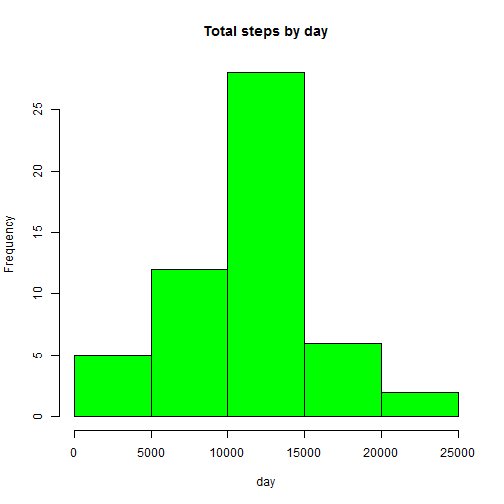
\includegraphics{README_files/figure-latex/unnamed-chunk-3-1.pdf}

\begin{Shaded}
\begin{Highlighting}[]
\CommentTok{#Histogram of total steps}
\KeywordTok{qplot}\NormalTok{(Q2}\OperatorTok{$}\StringTok{`}\DataTypeTok{Total Steps}\StringTok{`}\NormalTok{,}\DataTypeTok{geom=}\StringTok{"histogram"}\NormalTok{,}\DataTypeTok{xlab=}\StringTok{"Total Steps"}\NormalTok{,}\DataTypeTok{ylab=}\StringTok{"Counts"}\NormalTok{,}\DataTypeTok{main=}\StringTok{"Total Steps Historgram"}\NormalTok{,}\DataTypeTok{bins=}\DecValTok{7}\NormalTok{)}
\end{Highlighting}
\end{Shaded}

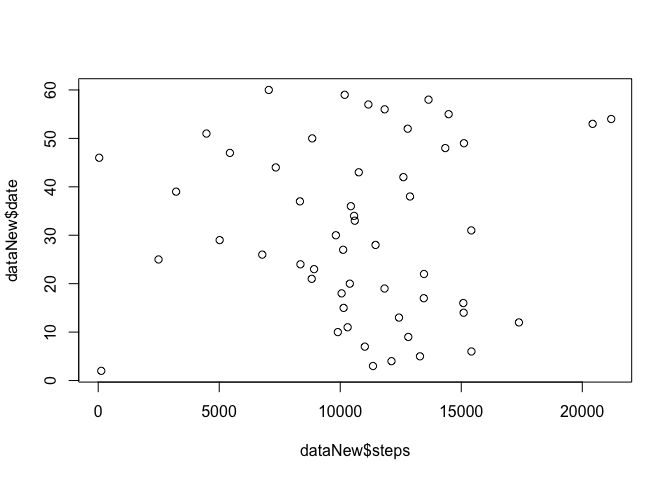
\includegraphics{README_files/figure-latex/unnamed-chunk-3-2.pdf}

\begin{verbatim}
## pdf 
##   2
\end{verbatim}

\begin{verbatim}
## `stat_bin()` using `bins = 30`. Pick better value with `binwidth`.
\end{verbatim}

\begin{verbatim}
## pdf 
##   2
\end{verbatim}

\hypertarget{step-3}{%
\subsection{Step 3}\label{step-3}}

\hypertarget{mean-and-median-number-of-steps-taken-each-day}{%
\subsubsection{Mean and median number of steps taken each
day}\label{mean-and-median-number-of-steps-taken-each-day}}

\begin{Shaded}
\begin{Highlighting}[]
\KeywordTok{library}\NormalTok{(dplyr)}
\end{Highlighting}
\end{Shaded}

\begin{verbatim}
## 
## Attaching package: 'dplyr'
\end{verbatim}

\begin{verbatim}
## The following objects are masked from 'package:stats':
## 
##     filter, lag
\end{verbatim}

\begin{verbatim}
## The following objects are masked from 'package:base':
## 
##     intersect, setdiff, setequal, union
\end{verbatim}

\begin{Shaded}
\begin{Highlighting}[]
\NormalTok{Q3<-}\KeywordTok{data.frame}\NormalTok{(}\KeywordTok{round}\NormalTok{(}\KeywordTok{tapply}\NormalTok{(activity}\OperatorTok{$}\NormalTok{steps,activity}\OperatorTok{$}\NormalTok{date,mean,}\DataTypeTok{na.rm=}\OtherTok{TRUE}\NormalTok{),}\DecValTok{2}\NormalTok{))}
\NormalTok{Q3}\OperatorTok{$}\NormalTok{date<-}\KeywordTok{rownames}\NormalTok{(Q3)}
\KeywordTok{rownames}\NormalTok{(Q3)<-}\OtherTok{NULL}
\KeywordTok{names}\NormalTok{(Q3)[[}\DecValTok{1}\NormalTok{]]<-}\StringTok{"Mean Steps"}
\NormalTok{temp<-activity}\OperatorTok\KeywordTok{select}\NormalTok{(date,steps) }\OperatorTok\StringTok{ }\KeywordTok{group_by}\NormalTok{(date) }\OperatorTok\StringTok{ }\KeywordTok{summarise}\NormalTok{(}\KeywordTok{median}\NormalTok{(steps))}
\end{Highlighting}
\end{Shaded}

\begin{verbatim}
## `summarise()` ungrouping output (override with `.groups` argument)
\end{verbatim}

\begin{Shaded}
\begin{Highlighting}[]
\KeywordTok{names}\NormalTok{(temp)[[}\DecValTok{2}\NormalTok{]]<-}\StringTok{"Median Steps"}
\NormalTok{Q3}\OperatorTok{$}\NormalTok{median<-temp}\OperatorTok{$}\StringTok{`}\DataTypeTok{Median Steps}\StringTok{`}
\NormalTok{Q3<-Q3 }\OperatorTok\StringTok{ }\KeywordTok{select}\NormalTok{(date,}\StringTok{`}\DataTypeTok{Mean Steps}\StringTok{`}\NormalTok{,median)}
\end{Highlighting}
\end{Shaded}

\hypertarget{step-4}{%
\subsection{Step 4}\label{step-4}}

\hypertarget{time-series-plot-of-the-average-number-of-steps-taken}{%
\subsubsection{Time series plot of the average number of steps
taken}\label{time-series-plot-of-the-average-number-of-steps-taken}}

\begin{Shaded}
\begin{Highlighting}[]
\NormalTok{Q4<-Q3}
\NormalTok{Q4}\OperatorTok{$}\NormalTok{date<-}\KeywordTok{as.Date}\NormalTok{(Q4}\OperatorTok{$}\NormalTok{date,}\DataTypeTok{format=}\StringTok{"%Y-%m-%d"}\NormalTok{)}
\KeywordTok{ggplot}\NormalTok{(Q4,}\KeywordTok{aes}\NormalTok{(}\DataTypeTok{x=}\NormalTok{Q4}\OperatorTok{$}\NormalTok{date,}\DataTypeTok{y=}\NormalTok{Q4}\OperatorTok{$}\StringTok{`}\DataTypeTok{Mean Steps}\StringTok{`}\NormalTok{))}\OperatorTok{+}\KeywordTok{geom_bar}\NormalTok{(}\DataTypeTok{stat=}\StringTok{"identity"}\NormalTok{)}\OperatorTok{+}\KeywordTok{scale_x_date}\NormalTok{()}\OperatorTok{+}\KeywordTok{ylab}\NormalTok{(}\StringTok{"Mean Steps Every day"}\NormalTok{)}\OperatorTok{+}\KeywordTok{xlab}\NormalTok{(}\StringTok{"Date"}\NormalTok{)}\OperatorTok{+}\KeywordTok{ggtitle}\NormalTok{(}\StringTok{"Mean Steps by Date"}\NormalTok{)}
\end{Highlighting}
\end{Shaded}

\begin{verbatim}
## Warning: Use of `Q4$date` is discouraged. Use `date` instead.
\end{verbatim}

\begin{verbatim}
## Warning: Use of `Q4$`Mean Steps`` is discouraged. Use `Mean Steps` instead.
\end{verbatim}

\begin{verbatim}
## Warning: Removed 8 rows containing missing values (position_stack).
\end{verbatim}

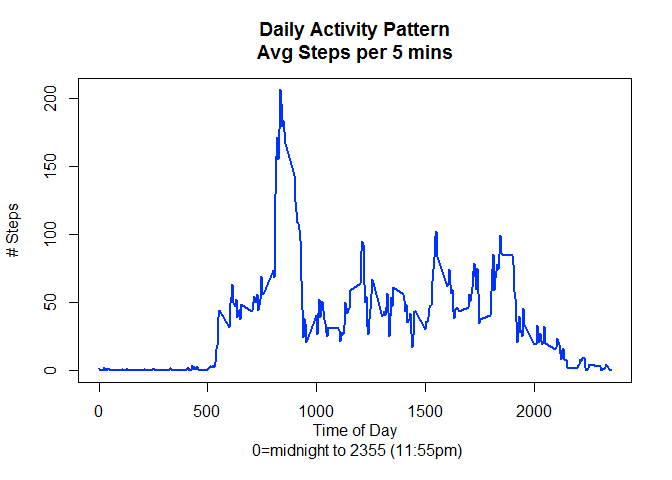
\includegraphics{README_files/figure-latex/unnamed-chunk-6-1.pdf}

\begin{verbatim}
## Warning: Use of `Q4$date` is discouraged. Use `date` instead.
\end{verbatim}

\begin{verbatim}
## Warning: Use of `Q4$`Mean Steps`` is discouraged. Use `Mean Steps` instead.
\end{verbatim}

\begin{verbatim}
## Warning: Removed 8 rows containing missing values (position_stack).
\end{verbatim}

\begin{verbatim}
## pdf 
##   2
\end{verbatim}

\hypertarget{step-5}{%
\subsection{Step 5}\label{step-5}}

\hypertarget{the-5-minute-interval-that-on-average-contains-the-maximum-number-of-steps}{%
\subsubsection{The 5-minute interval that, on average, contains the
maximum number of
steps}\label{the-5-minute-interval-that-on-average-contains-the-maximum-number-of-steps}}

\begin{Shaded}
\begin{Highlighting}[]
\CommentTok{#This is assuming that the words on average means averaging steps by date and interval}
\NormalTok{activity}\OperatorTok{$}\NormalTok{interval<-}\KeywordTok{factor}\NormalTok{(activity}\OperatorTok{$}\NormalTok{interval)}
\NormalTok{Q5<-}\KeywordTok{aggregate}\NormalTok{(}\DataTypeTok{data=}\NormalTok{activity,steps}\OperatorTok{~}\NormalTok{date}\OperatorTok{+}\NormalTok{interval,}\DataTypeTok{FUN=}\StringTok{"mean"}\NormalTok{)}
\NormalTok{Q5<-}\KeywordTok{aggregate}\NormalTok{(}\DataTypeTok{data=}\NormalTok{Q5,steps}\OperatorTok{~}\NormalTok{interval,}\DataTypeTok{FUN=}\StringTok{"max"}\NormalTok{)}
\end{Highlighting}
\end{Shaded}

\hypertarget{step-6}{%
\subsection{Step 6}\label{step-6}}

Code to describe and show a strategy for imputing missing data There are
multiple strategies to deal with multiple value imputations. The common
strategies include: 1. Constant value imputations 2. Regression model
value imputations 3. Mean/mode value substitutions For the purpose of
simplicity, in this question, I will use the mean/mode value
substitution strategy to impute missing values. That is, using the mean
values to substitute out the missing values in the original data set
Before doing any sort of imputation, it is helpful to understand what
are the distributions of missing values by date and interval

\begin{Shaded}
\begin{Highlighting}[]
\NormalTok{Q6<-activity}
\NormalTok{Q6}\OperatorTok{$}\NormalTok{Missing<-}\KeywordTok{is.na}\NormalTok{(Q6}\OperatorTok{$}\NormalTok{steps)}
\NormalTok{Q6<-}\KeywordTok{aggregate}\NormalTok{(}\DataTypeTok{data=}\NormalTok{Q6,Missing}\OperatorTok{~}\NormalTok{date}\OperatorTok{+}\NormalTok{interval,}\DataTypeTok{FUN=}\StringTok{"sum"}\NormalTok{)}
\NormalTok{Q6}\FloatTok{.1}\NormalTok{<-}\KeywordTok{data.frame}\NormalTok{(}\KeywordTok{tapply}\NormalTok{(Q6}\OperatorTok{$}\NormalTok{Missing,Q6}\OperatorTok{$}\NormalTok{date,sum))}
\NormalTok{Q6}\FloatTok{.1}\OperatorTok{$}\NormalTok{date<-}\KeywordTok{rownames}\NormalTok{(Q6}\FloatTok{.1}\NormalTok{)}
\KeywordTok{rownames}\NormalTok{(Q6}\FloatTok{.1}\NormalTok{)<-}\OtherTok{NULL}
\KeywordTok{names}\NormalTok{(Q6}\FloatTok{.1}\NormalTok{)<-}\KeywordTok{c}\NormalTok{(}\StringTok{"Missing"}\NormalTok{,}\StringTok{"date"}\NormalTok{)}
\NormalTok{Q6}\FloatTok{.1}\OperatorTok{$}\NormalTok{date<-}\KeywordTok{as.Date}\NormalTok{(Q6}\FloatTok{.1}\OperatorTok{$}\NormalTok{date,}\DataTypeTok{format=}\StringTok{"%Y-%m-%d"}\NormalTok{)}
\NormalTok{Q6}\FloatTok{.2}\NormalTok{<-}\KeywordTok{data.frame}\NormalTok{(}\KeywordTok{tapply}\NormalTok{(Q6}\OperatorTok{$}\NormalTok{Missing,Q6}\OperatorTok{$}\NormalTok{interval,sum))}
\NormalTok{Q6}\FloatTok{.2}\OperatorTok{$}\NormalTok{date<-}\KeywordTok{rownames}\NormalTok{(Q6}\FloatTok{.2}\NormalTok{)}
\KeywordTok{rownames}\NormalTok{(Q6}\FloatTok{.2}\NormalTok{)<-}\OtherTok{NULL}
\KeywordTok{names}\NormalTok{(Q6}\FloatTok{.2}\NormalTok{)<-}\KeywordTok{c}\NormalTok{(}\StringTok{"Missing"}\NormalTok{,}\StringTok{"Interval"}\NormalTok{)}
\KeywordTok{par}\NormalTok{(}\DataTypeTok{mfrow=}\KeywordTok{c}\NormalTok{(}\DecValTok{1}\NormalTok{,}\DecValTok{2}\NormalTok{))}
\KeywordTok{plot}\NormalTok{(}\DataTypeTok{y=}\NormalTok{Q6}\FloatTok{.1}\OperatorTok{$}\NormalTok{Missing,}\DataTypeTok{x=}\NormalTok{Q6}\FloatTok{.1}\OperatorTok{$}\NormalTok{date,}\DataTypeTok{main=}\StringTok{"Missing Value Distribution by Date"}\NormalTok{)}
\KeywordTok{plot}\NormalTok{(}\DataTypeTok{y=}\NormalTok{Q6}\FloatTok{.2}\OperatorTok{$}\NormalTok{Missing,}\DataTypeTok{x=}\NormalTok{Q6}\FloatTok{.2}\OperatorTok{$}\NormalTok{Interval,}\DataTypeTok{main=}\StringTok{"Missing Value Distribution by Interval"}\NormalTok{)}
\end{Highlighting}
\end{Shaded}

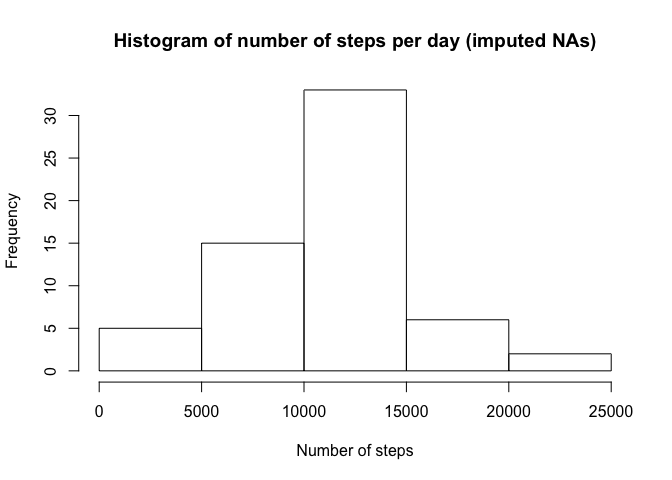
\includegraphics{README_files/figure-latex/unnamed-chunk-9-1.pdf}

\begin{Shaded}
\begin{Highlighting}[]
\KeywordTok{table}\NormalTok{(activity}\OperatorTok{$}\NormalTok{date)}
\end{Highlighting}
\end{Shaded}

\begin{verbatim}
## 
## 2012-10-01 2012-10-02 2012-10-03 2012-10-04 2012-10-05 2012-10-06 2012-10-07 
##        288        288        288        288        288        288        288 
## 2012-10-08 2012-10-09 2012-10-10 2012-10-11 2012-10-12 2012-10-13 2012-10-14 
##        288        288        288        288        288        288        288 
## 2012-10-15 2012-10-16 2012-10-17 2012-10-18 2012-10-19 2012-10-20 2012-10-21 
##        288        288        288        288        288        288        288 
## 2012-10-22 2012-10-23 2012-10-24 2012-10-25 2012-10-26 2012-10-27 2012-10-28 
##        288        288        288        288        288        288        288 
## 2012-10-29 2012-10-30 2012-10-31 2012-11-01 2012-11-02 2012-11-03 2012-11-04 
##        288        288        288        288        288        288        288 
## 2012-11-05 2012-11-06 2012-11-07 2012-11-08 2012-11-09 2012-11-10 2012-11-11 
##        288        288        288        288        288        288        288 
## 2012-11-12 2012-11-13 2012-11-14 2012-11-15 2012-11-16 2012-11-17 2012-11-18 
##        288        288        288        288        288        288        288 
## 2012-11-19 2012-11-20 2012-11-21 2012-11-22 2012-11-23 2012-11-24 2012-11-25 
##        288        288        288        288        288        288        288 
## 2012-11-26 2012-11-27 2012-11-28 2012-11-29 2012-11-30 
##        288        288        288        288        288
\end{verbatim}

By this point, from the plot, that the missing values have a very
disctinct pattern. For every interval, there are consistantly 8 missing
values. For the date, there are consistantly 288 missing values. And in
total, there are 8 dates that have missing value. We don't exactly know
the cause for these missing values but there's a pattern. For that
matter, we can see that the mean value imputation is appropriate.

We can see that every date has 288 data points. It means that the 8
dates have no data points at all what so ever. We can refine the
analysis by looking at these missing values depending on their Weekday
and interval parameters to matach with the average

\begin{Shaded}
\begin{Highlighting}[]
\CommentTok{#Dates that have missing values }
\KeywordTok{library}\NormalTok{(lubridate)}
\NormalTok{Q6}\FloatTok{.3}\NormalTok{<-}\KeywordTok{as.data.frame}\NormalTok{(Q6}\FloatTok{.1}\NormalTok{) }\OperatorTok\StringTok{ }\KeywordTok{select}\NormalTok{(date,Missing) }\OperatorTok\StringTok{ }\KeywordTok{arrange}\NormalTok{(}\KeywordTok{desc}\NormalTok{(Missing))}
\NormalTok{Q6}\FloatTok{.3}\NormalTok{<-Q6}\FloatTok{.3}\NormalTok{[}\KeywordTok{which}\NormalTok{(Q6}\FloatTok{.3}\OperatorTok{$}\NormalTok{Missing}\OperatorTok{!=}\DecValTok{0}\NormalTok{),]}
\NormalTok{Q6}\FloatTok{.3}\OperatorTok{$}\NormalTok{Weekday<-}\KeywordTok{wday}\NormalTok{(Q6}\FloatTok{.3}\OperatorTok{$}\NormalTok{date,}\DataTypeTok{label=}\OtherTok{TRUE}\NormalTok{)}
\NormalTok{Q6}\FloatTok{.4}\NormalTok{<-activity}
\NormalTok{Q6}\FloatTok{.4}\OperatorTok{$}\NormalTok{weekday<-}\KeywordTok{wday}\NormalTok{(Q6}\FloatTok{.4}\OperatorTok{$}\NormalTok{date,}\DataTypeTok{label=}\OtherTok{TRUE}\NormalTok{)}
\CommentTok{#Finding the mean of steps every monday, and every interval}
\NormalTok{Q6}\FloatTok{.5}\NormalTok{<-}\KeywordTok{aggregate}\NormalTok{(}\DataTypeTok{data=}\NormalTok{Q6}\FloatTok{.4}\NormalTok{,steps}\OperatorTok{~}\NormalTok{interval}\OperatorTok{+}\NormalTok{weekday,}\DataTypeTok{FUN=}\StringTok{"mean"}\NormalTok{,}\DataTypeTok{na.rm=}\OtherTok{TRUE}\NormalTok{)}
\CommentTok{#Merge the pre-imputation table Q6.4 table with the average table Q6.5}
\NormalTok{Q6}\FloatTok{.6}\NormalTok{<-}\KeywordTok{merge}\NormalTok{(}\DataTypeTok{x=}\NormalTok{Q6}\FloatTok{.4}\NormalTok{,}\DataTypeTok{y=}\NormalTok{Q6}\FloatTok{.5}\NormalTok{,}\DataTypeTok{by.x=}\KeywordTok{c}\NormalTok{(}\StringTok{"interval"}\NormalTok{,}\StringTok{"weekday"}\NormalTok{),}\DataTypeTok{by.y=}\KeywordTok{c}\NormalTok{(}\StringTok{"interval"}\NormalTok{,}\StringTok{"weekday"}\NormalTok{),}\DataTypeTok{all.x=}\OtherTok{TRUE}\NormalTok{)}
\CommentTok{#Conditionally replacing the steps.x column NA value with the values from steps.y column value }
\NormalTok{Q6}\FloatTok{.6}\OperatorTok{$}\NormalTok{Steps.Updated<-}\DecValTok{0}
\ControlFlowTok{for}\NormalTok{ (i }\ControlFlowTok{in} \DecValTok{1}\OperatorTok{:}\KeywordTok{dim}\NormalTok{(Q6}\FloatTok{.6}\NormalTok{)[[}\DecValTok{1}\NormalTok{]])\{}
\ControlFlowTok{if}\NormalTok{(}\KeywordTok{is.na}\NormalTok{(Q6}\FloatTok{.6}\NormalTok{[i,}\DecValTok{3}\NormalTok{]))\{Q6}\FloatTok{.6}\NormalTok{[i,}\DecValTok{6}\NormalTok{]=Q6}\FloatTok{.6}\NormalTok{[i,}\DecValTok{5}\NormalTok{]\}}
\ControlFlowTok{else}\NormalTok{ \{Q6}\FloatTok{.6}\NormalTok{[i,}\DecValTok{6}\NormalTok{]=Q6}\FloatTok{.6}\NormalTok{[i,}\DecValTok{3}\NormalTok{]\}}
\NormalTok{\}}
\CommentTok{#Now simplify the imputed analytical data frame}
\NormalTok{Q6}\FloatTok{.6}\NormalTok{ <-Q6}\FloatTok{.6}  \OperatorTok\StringTok{ }\KeywordTok{select}\NormalTok{(date,weekday,interval,Steps.Updated)}
\KeywordTok{names}\NormalTok{(Q6}\FloatTok{.6}\NormalTok{)[[}\DecValTok{4}\NormalTok{]]<-}\StringTok{"Steps"}
\end{Highlighting}
\end{Shaded}

\hypertarget{step-7}{%
\subsection{Step 7}\label{step-7}}

\hypertarget{histogram-of-the-total-number-of-steps-taken-each-day-after-missing-values-are-imputed}{%
\subsubsection{Histogram of the total number of steps taken each day
after missing values are
imputed}\label{histogram-of-the-total-number-of-steps-taken-each-day-after-missing-values-are-imputed}}

\begin{Shaded}
\begin{Highlighting}[]
\KeywordTok{qplot}\NormalTok{(Q6}\FloatTok{.6}\OperatorTok{$}\NormalTok{Steps,}\DataTypeTok{geom=}\StringTok{"histogram"}\NormalTok{,}\DataTypeTok{main=}\StringTok{"Total steps taken histogram post imputation"}\NormalTok{,}\DataTypeTok{xlab=}\StringTok{"Steps"}\NormalTok{,}\DataTypeTok{ylab=}\StringTok{"Count"}\NormalTok{)}
\end{Highlighting}
\end{Shaded}

\begin{verbatim}
## `stat_bin()` using `bins = 30`. Pick better value with `binwidth`.
\end{verbatim}

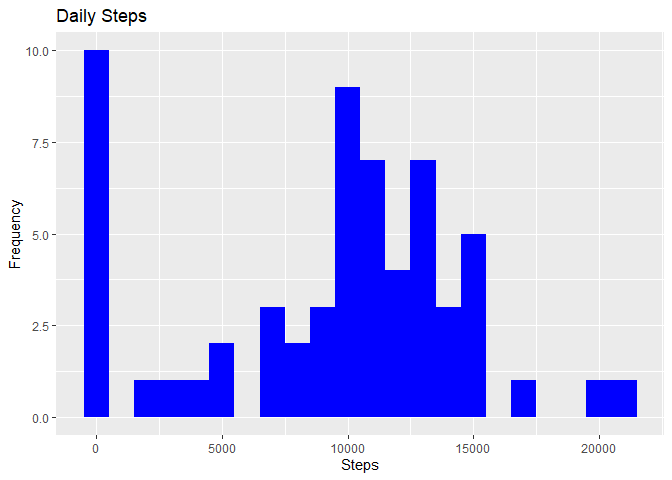
\includegraphics{README_files/figure-latex/unnamed-chunk-11-1.pdf}

\begin{verbatim}
## `stat_bin()` using `bins = 30`. Pick better value with `binwidth`.
\end{verbatim}

\begin{verbatim}
## pdf 
##   2
\end{verbatim}

\hypertarget{step-8}{%
\subsection{Step 8}\label{step-8}}

\hypertarget{panel-plot-comparing-the-average-number-of-steps-taken-per-5-minute-interval-across-weekdays-and-weekends}{%
\subsubsection{Panel plot comparing the average number of steps taken
per 5-minute interval across weekdays and
weekends}\label{panel-plot-comparing-the-average-number-of-steps-taken-per-5-minute-interval-across-weekdays-and-weekends}}

\begin{Shaded}
\begin{Highlighting}[]
\NormalTok{Q8<-Q6}\FloatTok{.6}
\KeywordTok{levels}\NormalTok{(Q8}\OperatorTok{$}\NormalTok{weekday)<-}\KeywordTok{c}\NormalTok{(}\DecValTok{1}\NormalTok{,}\DecValTok{2}\NormalTok{,}\DecValTok{3}\NormalTok{,}\DecValTok{4}\NormalTok{,}\DecValTok{5}\NormalTok{,}\DecValTok{6}\NormalTok{,}\DecValTok{7}\NormalTok{)}
\NormalTok{Q8}\OperatorTok{$}\NormalTok{WDWE<-Q8}\OperatorTok{$}\NormalTok{weekday }\OperatorTok\StringTok{ }\KeywordTok{c}\NormalTok{(}\DecValTok{1}\NormalTok{,}\DecValTok{2}\NormalTok{,}\DecValTok{3}\NormalTok{,}\DecValTok{4}\NormalTok{,}\DecValTok{5}\NormalTok{)}
\NormalTok{Q8}\FloatTok{.1}\NormalTok{<-}\KeywordTok{aggregate}\NormalTok{(}\DataTypeTok{data=}\NormalTok{Q8,Steps}\OperatorTok{~}\NormalTok{interval}\OperatorTok{+}\NormalTok{WDWE,mean,}\DataTypeTok{na.rm=}\OtherTok{TRUE}\NormalTok{)}
\NormalTok{Q8}\FloatTok{.1}\OperatorTok{$}\NormalTok{WDWE<-}\KeywordTok{as.factor}\NormalTok{(Q8}\FloatTok{.1}\OperatorTok{$}\NormalTok{WDWE)}
\KeywordTok{levels}\NormalTok{(Q8}\FloatTok{.1}\OperatorTok{$}\NormalTok{WDWE)<-}\KeywordTok{c}\NormalTok{(}\StringTok{"Weekend"}\NormalTok{,}\StringTok{"Weekday"}\NormalTok{)}
\KeywordTok{ggplot}\NormalTok{(}\DataTypeTok{data=}\NormalTok{Q8}\FloatTok{.1}\NormalTok{,}\KeywordTok{aes}\NormalTok{(}\DataTypeTok{y=}\NormalTok{Steps,}\DataTypeTok{x=}\NormalTok{interval,}\DataTypeTok{group=}\DecValTok{1}\NormalTok{,}\DataTypeTok{color=}\NormalTok{WDWE))}\OperatorTok{+}\KeywordTok{geom_line}\NormalTok{() }\OperatorTok{+}\KeywordTok{scale_x_discrete}\NormalTok{(}\DataTypeTok{breaks =} \KeywordTok{seq}\NormalTok{(}\DecValTok{0}\NormalTok{, }\DecValTok{2500}\NormalTok{, }\DataTypeTok{by =} \DecValTok{300}\NormalTok{))}\OperatorTok{+}\KeywordTok{ylab}\NormalTok{(}\StringTok{"Mean Steps"}\NormalTok{)}\OperatorTok{+}\KeywordTok{xlab}\NormalTok{(}\StringTok{"Intervals"}\NormalTok{)}\OperatorTok{+}\KeywordTok{ggtitle}\NormalTok{(}\StringTok{"Mean steps across intervals by Weekend and Weekday"}\NormalTok{)}
\end{Highlighting}
\end{Shaded}

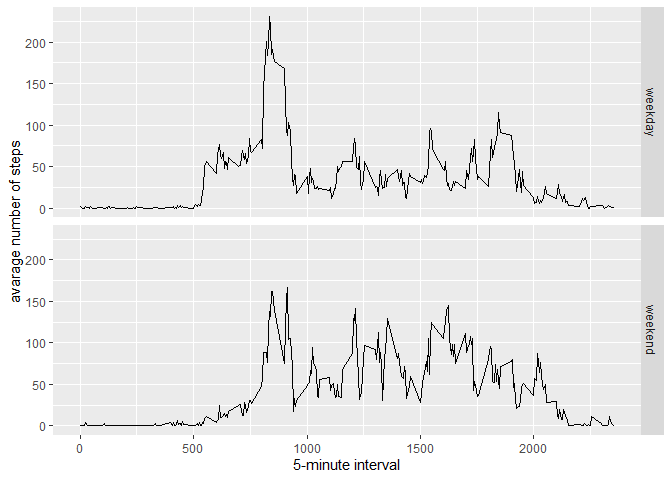
\includegraphics{README_files/figure-latex/unnamed-chunk-13-1.pdf}

\begin{Shaded}
\begin{Highlighting}[]
\CommentTok{#Producing the panel plot}
\NormalTok{Q8}\FloatTok{.1}\OperatorTok{$}\NormalTok{interval<-}\KeywordTok{as.numeric}\NormalTok{(}\KeywordTok{as.character}\NormalTok{(Q8}\FloatTok{.1}\OperatorTok{$}\NormalTok{interval))}
\KeywordTok{library}\NormalTok{(lattice)}
\KeywordTok{xyplot}\NormalTok{(}\DataTypeTok{data=}\NormalTok{Q8}\FloatTok{.1}\NormalTok{,Steps}\OperatorTok{~}\NormalTok{interval}\OperatorTok{|}\NormalTok{WDWE, }\DataTypeTok{grid =} \OtherTok{TRUE}\NormalTok{, }\DataTypeTok{type =} \KeywordTok{c}\NormalTok{(}\StringTok{"p"}\NormalTok{, }\StringTok{"smooth"}\NormalTok{), }\DataTypeTok{lwd =} \DecValTok{4}\NormalTok{,}\DataTypeTok{panel =}\NormalTok{ panel.smoothScatter)}
\end{Highlighting}
\end{Shaded}

\begin{verbatim}
## (loaded the KernSmooth namespace)
\end{verbatim}

\includegraphics{README_files/figure-latex/unnamed-chunk-13-2.pdf}

\begin{Shaded}
\begin{Highlighting}[]
\KeywordTok{library}\NormalTok{(hexbin)}
\KeywordTok{hexbinplot}\NormalTok{(}\DataTypeTok{data=}\NormalTok{Q8}\FloatTok{.1}\NormalTok{,Steps}\OperatorTok{~}\NormalTok{interval}\OperatorTok{|}\NormalTok{WDWE, }\DataTypeTok{aspect =} \DecValTok{1}\NormalTok{, }\DataTypeTok{bins=}\DecValTok{50}\NormalTok{)}
\end{Highlighting}
\end{Shaded}

\includegraphics{README_files/figure-latex/unnamed-chunk-13-3.pdf}

\begin{verbatim}
## pdf 
##   2
\end{verbatim}

\begin{verbatim}
## pdf 
##   2
\end{verbatim}

\begin{verbatim}
## pdf 
##   2
\end{verbatim}

\end{document}
